\subsection{Zoom}

The last alteration analyzed is the zoom. \Fig~\ref{fig:acc_zo_wu} illustrates how the accuracy changes with altered data by the zoom. The accuracy of both networks starts to decrease as soon as the zoom level is increased, suggesting a poor robustness to this alteration.

The last alteration under examination is the zoom. In \Fig~\ref{fig:acc_zo_wu}, it is possible to observe how the accuracy is affected by varying levels of zoom. Notably, as the zoom level increases, the accuracy of both networks begins to decline, indicating a lack of robustness against this alteration.

\begin{figure}[h]
	\centering
	\begin{subfigure}{.5\textwidth}
		\centering
		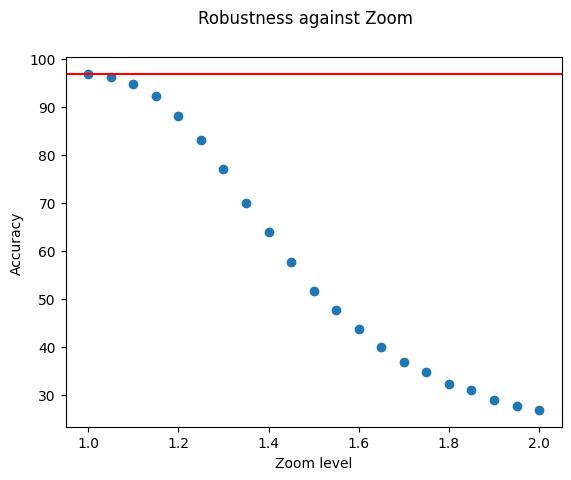
\includegraphics[width=0.9\linewidth]{ImageFiles/EvalBNN/ZO/WU/acc}
		\caption{BNN}
		\label{fig:zo_acc_wu_bnn}
	\end{subfigure}%
	\begin{subfigure}{.5\textwidth}
		\centering
		us		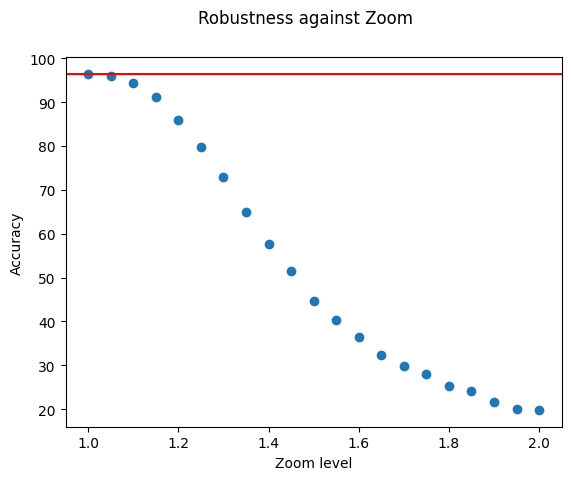
\includegraphics[width=0.9\linewidth]{ImageFiles/EvalANN/zoom_ann}
		\caption{Standard NN}
		\label{fig:zoom_ann}
	\end{subfigure}
	\caption{Accuracy trend for zoom}
	\label{fig:acc_zo_wu}
\end{figure}

The poor robustness is confirmed by the quantitative metrics computed, which are $0.7731$ for the BNN and $0.7467$ for the standard NN.

The uncertainties estimated by the BNN exhibit a defined pattern in this case, as depicted in \Fig~\ref{fig:zo_uncertainty}. Specifically, the aleatoric uncertainty, shown in \Fig~\ref{fig:zo_aleatoric}, follows an exponential trend, reaching a saturation level around a zoom level of $1.4$. On the other hand, epistemic uncertainty, illustrated in \Fig~\ref{fig:zo_epistemic}, reflects the trend of accuracy. In essence, as the zoom level increases, the network becomes progressively less confident in its predictions.

\begin{figure}[h]
	\centering
	\begin{subfigure}{.5\textwidth}
		\centering
		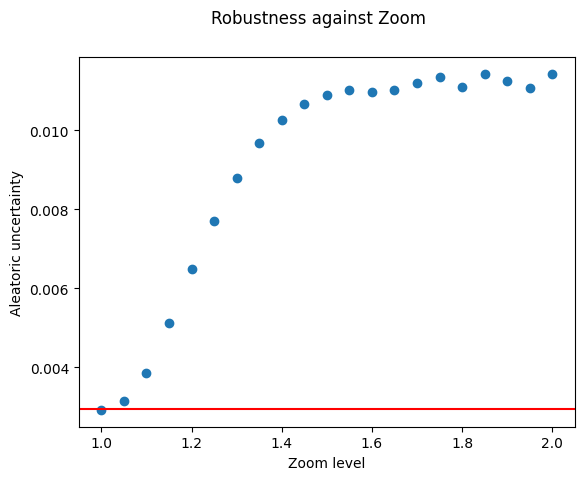
\includegraphics[width=0.9\linewidth]{ImageFiles/EvalBNN/ZO/aleatoric}
		\caption{Aleatoric uncertainty}
		\label{fig:zo_aleatoric}
	\end{subfigure}%
	\begin{subfigure}{.5\textwidth}
		\centering
		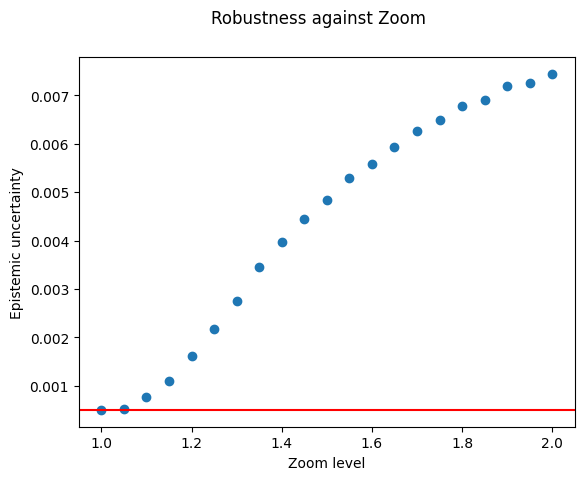
\includegraphics[width=0.9\linewidth]{ImageFiles/EvalBNN/ZO/epistemic}
		\caption{Epistemic uncertainty}
		\label{fig:zo_epistemic}
	\end{subfigure}
	\caption{Uncertainty trend for zoom}
	\label{fig:zo_uncertainty}
\end{figure}

\vspace{0.3cm}
\textbf{Classification using aleatoric uncertainty}
\vspace{0.1cm}

The utilization of aleatoric uncertainty yields the results shown in \Fig~\ref{fig:zo_au}. \Fig~\ref{fig:zo_au_acc} indicates a slight improvement in accuracy. However, there is a substantial increase in the unknown ratio, as depicted in \Fig~\ref{fig:zo_au_unkn}. This trade-off between accuracy and unknown ratio is further illustrated in \Fig~\ref{fig:zo_au_eff}, where the effectiveness metric reflects the degradation in performance.

\begin{figure}[h]
	\centering
	\begin{subfigure}{.33\textwidth}
		\centering
		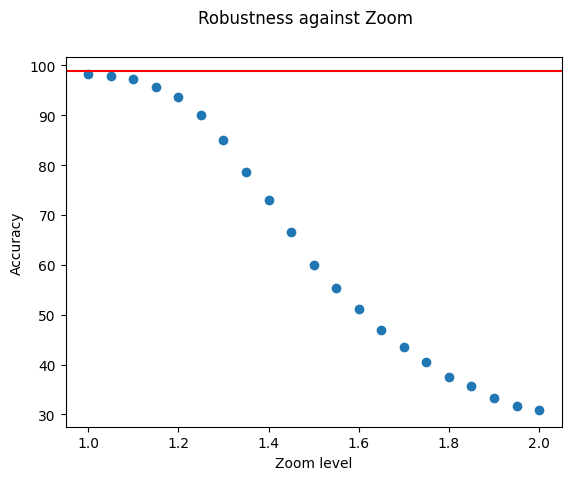
\includegraphics[width=0.9\linewidth]{ImageFiles/EvalBNN/ZO/AU/acc}
		\caption{Accuracy using aleatoric \\ uncertainty}
		\label{fig:zo_au_acc}
	\end{subfigure}%
	\begin{subfigure}{.33\textwidth}
		\centering
		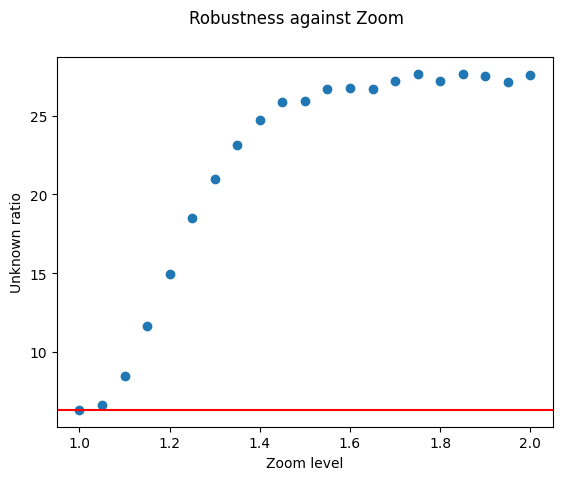
\includegraphics[width=0.9\linewidth]{ImageFiles/EvalBNN/ZO/AU/unkn}
		\caption{Unknown ratio using aleatoric uncertainty}
		\label{fig:zo_au_unkn}
	\end{subfigure}%
	\begin{subfigure}{.33\textwidth}
		\centering
		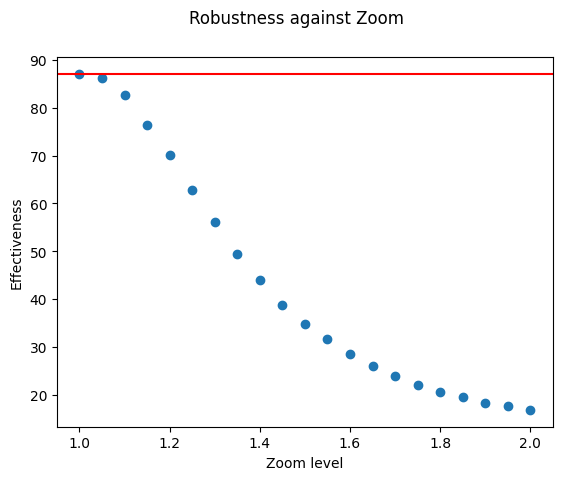
\includegraphics[width=0.9\linewidth]{ImageFiles/EvalBNN/ZO/AU/eff}
		\caption{Effectiveness using aleatoric uncertainty}
		\label{fig:zo_au_eff}
	\end{subfigure}
	\caption{Robustness graph for zoom when aleatoric uncertainty is employed in the classification}
	\label{fig:zo_au}
\end{figure}


\Tab~\ref{table:rob_zo_au} provides the quantitative robustness measurements. While there is a slight improvement in accuracy reflected in the $rob$ metric, the augmented robustness metric demonstrates the poor performance due to the substantial increase in the unknown ratio.

\begin{table}[h]
	\centering
	\begin{tabular}{|| l | l ||} 
		\hline
		\textbf{Parameter} & \textbf{Value} \\
		\hline
		\hline
		$rob_{Zoom}$ & $0.7950$ \\
		$robInd_{Zoom}$ & $0.8901$ \\
		$robAug_{Zoom}$ & $0.7209$ \\	
		\hline
	\end{tabular}	
	\caption{Robustness metrics for zoom when the aleatoric uncertainty is employed}
	\label{table:rob_zo_au}
\end{table}

\vspace{0.3cm}
\textbf{Classification using epistemic uncertainty}
\vspace{0.1cm}

The outcomes obtained using epistemic uncertainty are displayed in \Fig~\ref{fig:zo_au}. An important observation relates to the unknown ratio, depicted in \Fig~\ref{fig:zo_au_unkn}, which reaches values of approximately $40\%$. This implies that roughly half of the predictions are classified as unknown. However, despite this, the accuracy, shown in \Fig~\ref{fig:zo_au_acc}, does not exhibit any improvement. This underscores, once again, the ineffectiveness of epistemic uncertainty in identifying uncertain situations and enhancing robustness.

\begin{figure}[h]
	\centering
	\begin{subfigure}{.33\textwidth}
		\centering
		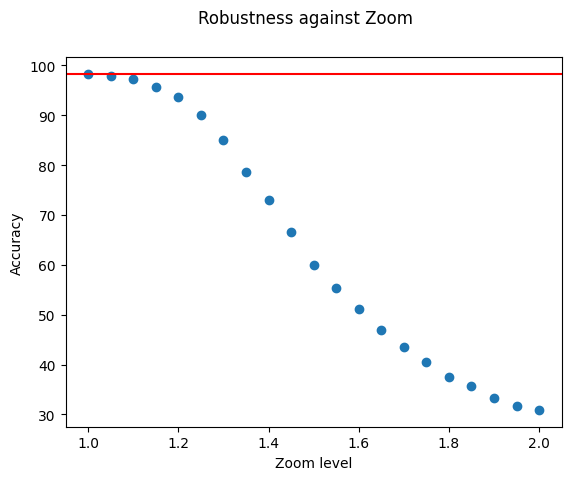
\includegraphics[width=0.9\linewidth]{ImageFiles/EvalBNN/ZO/EU/acc}
		\caption{Accuracy using epistemic \\ uncertainty}
		\label{fig:zo_eu_acc}
	\end{subfigure}%
	\begin{subfigure}{.33\textwidth}
		\centering
		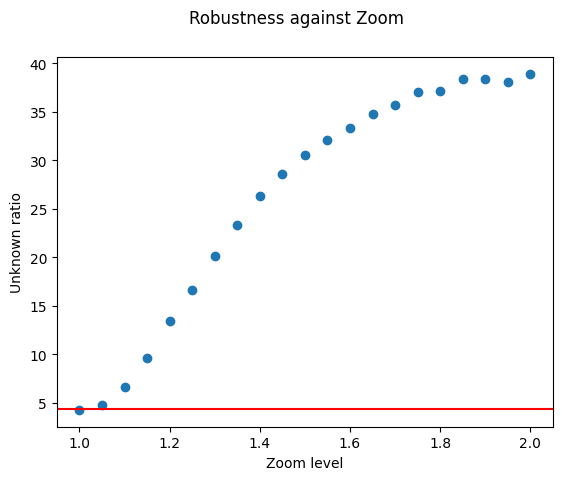
\includegraphics[width=0.9\linewidth]{ImageFiles/EvalBNN/ZO/EU/unkn}
		\caption{Unknown ratio using \\ epistemic uncertainty}
		\label{fig:zo_eu_unkn}
	\end{subfigure}%
	\begin{subfigure}{.33\textwidth}
		\centering
		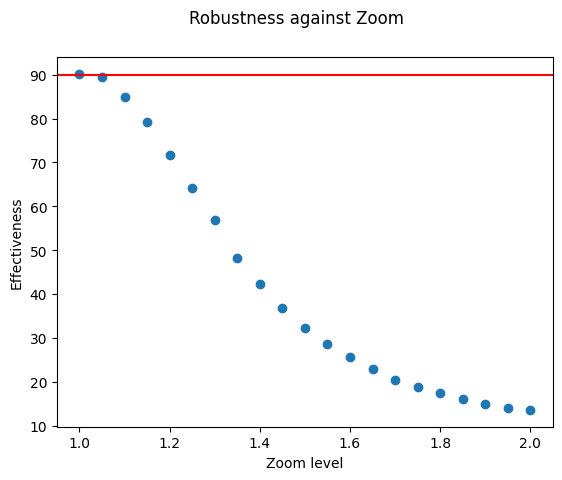
\includegraphics[width=0.9\linewidth]{ImageFiles/EvalBNN/ZO/EU/eff}
		\caption{Effectiveness using \\ epistemic uncertainty}
		\label{fig:zo_eu_eff}
	\end{subfigure}
	\caption{Robustness graph for zoom when epistemic uncertainty is employed in the classification}
	\label{fig:zo_eu}
\end{figure}

\Tab~\ref{table:rob_zo_eu} displays the robustness metrics.

\begin{table}[h]
	\centering
	\begin{tabular}{|| l | l ||} 
		\hline
		\textbf{Parameter} & \textbf{Value} \\
		\hline
		\hline
		$rob_{Zoom}$ & $0.7988$ \\
		$robInd_{Zoom}$ & $0.8560$ \\
		$robAug_{Zoom}$ & $0.7058$ \\	
		\hline
	\end{tabular}	
	\caption{Robustness metrics for zoom alteration when the epistemic uncertainty is employed}
	\label{table:rob_zo_eu}
\end{table}

\vspace{0.3cm}
\textbf{Classification using standard deviation}
\vspace{0.1cm}

The results obtained when using standard deviation, as illustrated in \Fig~\ref{fig:zo_vu}, exhibit the same behavior as when using aleatoric uncertainty. As always, the standard deviation is more pessimistic, leading to a better trend in accuracy, \Fig~\ref{fig:zo_vu_acc}, but balanced by a high unknown ratio, \Fig~\ref{fig:zo_vu_unkn}.

\Fig~\ref{fig:zo_vu} exhibits the same behavior as when using aleatoric uncertainty. As usual, the standard deviation is more pessimistic, leading to a better trend in accuracy, \Fig~\ref{fig:zo_vu_acc}, but this is balanced by a high unknown ratio, seen in \Fig~\ref{fig:zo_vu_unkn}.

\begin{figure}[h]
	\centering
	\begin{subfigure}{.33\textwidth}
		\centering
		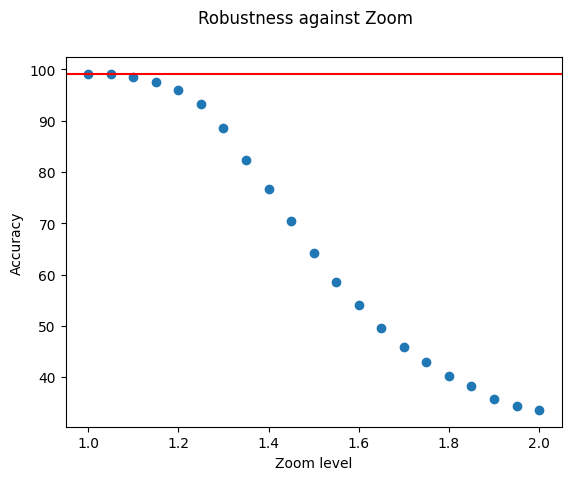
\includegraphics[width=0.9\linewidth]{ImageFiles/EvalBNN/ZO/VU/acc}
		\caption{Accuracy using standard \\ deviation}
		\label{fig:zo_vu_acc}
	\end{subfigure}%
	\begin{subfigure}{.33\textwidth}
		\centering
		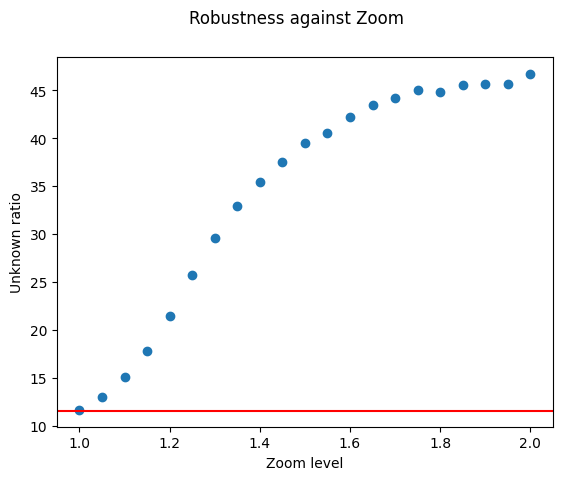
\includegraphics[width=0.9\linewidth]{ImageFiles/EvalBNN/ZO/VU/unkn}
		\caption{Unknown ratio using \\ standard deviation}
		\label{fig:zo_vu_unkn}
	\end{subfigure}%
	\begin{subfigure}{.33\textwidth}
		\centering
		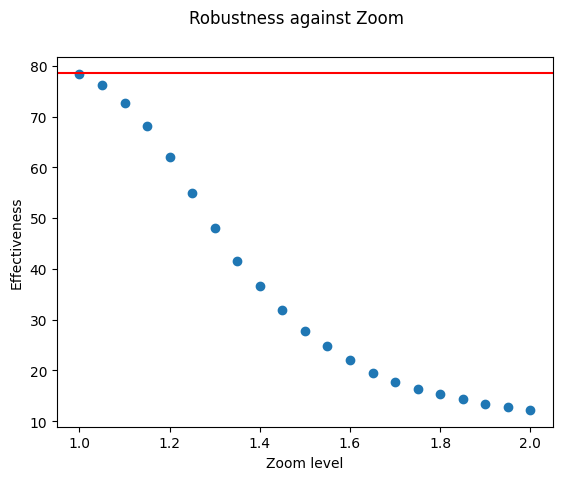
\includegraphics[width=0.9\linewidth]{ImageFiles/EvalBNN/ZO/VU/eff}
		\caption{Effectiveness using standard deviation}
		\label{fig:zo_vu_eff}
	\end{subfigure}
	\caption{Robustness graph for zoom when standard deviation is employed in the classification}
	\label{fig:zo_vu}
\end{figure}

\Tab~\ref{table:rob_zo_vu} gives the quantitative robustness measurements.

\begin{table}[h]
	\centering
	\begin{tabular}{|| l | l ||} 
		\hline
		\textbf{Parameter} & \textbf{Value} \\
		\hline
		\hline
		$rob_{Zoom}$ & $0.8101$ \\
		$robInd_{Zoom}$ & $0.8432$ \\
		$robAug_{Zoom}$ & $0.7031$ \\	
		\hline
	\end{tabular}	
	\caption{Robustness metrics for zoom when the standard deviation is employed}
	\label{table:rob_zo_vu}
\end{table}

\vspace{0.3cm}
\textbf{Comparison}
\vspace{0.1cm}

\Tab~\ref{table:rob_zo} provides a summary of the computed metrics. It is evident that the network is not robust against this alteration. In particular, the augmented robustness reflects the trade-off between accuracy and unknown ratio. In this scenario, aleatoric uncertainty provides the best $robAug$, while epistemic uncertainty demonstrates its inability to detect uncertain situations.

\begin{table}[h]
	\centering
	\begin{tabular}{|| l | l | l | l ||} 
		\hline
		\textbf{Parameter} & \textbf{Aleatoric} & \textbf{Epistemic} & \textbf{Standard deviation} \\
		\hline
		\hline
		$rob_{Zoom}$ & $0.7950$ & $0.7988$ & $0.8101$ \\
		$robInd_{Zoom}$ & $0.8901$ & $0.8560$ & $0.8432$ \\
		$robAug_{Zoom}$ & $0.7209$ & $0.7058$ & $0.7031$ \\	
		\hline
	\end{tabular}	
	\caption{Summary of the robustness metrics for zoom}
	\label{table:rob_zo}
\end{table}